\chapter{Theoretical Background and Literature}\label{Sec:Theory_and_Literature}

\section{Bose-Hubbard Model}\label{Sec:BHM_Theory}
The Hamiltonian investigated throughout this project is the Bose-Hubbard (BH) model:
\begin{subequations}\label{Eq:BHM}
\begin{equation}
    H = H_J + H_U
\end{equation}
\begin{equation}\label{Eq:HoppingHamiltonian}
    H_J = -J\sum_{\langle ij \rangle}b_{i}^{\dag}b_{j} + \text{H.c.}
\end{equation}
\begin{equation}\label{Eq:InteractionHamiltonian}
    H_U = \frac{U}{2}\sum_{i}n_{i}(n_{i}-1)
\end{equation}
\end{subequations}
Hats are omitted from operators. $b_{i}^\dag$ and $b_{i}$ are bosonic creation and annihilation operators, and $n_i=b_{i}^{\dag}b_{i}$ the number operator, at site $i$. $H_J$ represents hopping between all nearest-neighbour sites $\langle ij \rangle$ with amplitude $J\geq0$. $H_U$ is the on-site repulsive interaction energy between particles with strength $U\geq0$. The ratio $U/J$ determines the behaviour regime; $J$ was set to 1 throughout the project. The BH model neglects hoppings to beyond-nearest-neighbour sites, interactions between particles on different sites, and assumes contact interactions (\textit{s}-wave scattering). These approximations are all appropriate for cold atoms in a sufficiently deep optical potential \cite{Jaksch}.

\section{Kagome Lattice and Bandstructure}\label{Sec:Kagome_FB_Theory}

The kagome lattice (Fig. \ref{Fig:Lattice_Structure}) is a hexagonal Bravais lattice, with a triangular three-site basis in each unit cell. The lattice vectors are $\textbf{a}_1=a(1,0)$ and $\textbf{a}_2=a(1/2,\sqrt{3}/2)$, with $a$ the lattice constant.

\vspace{1cm}

\begin{figure}[ht]
    \centering
    \sidesubfloat[]{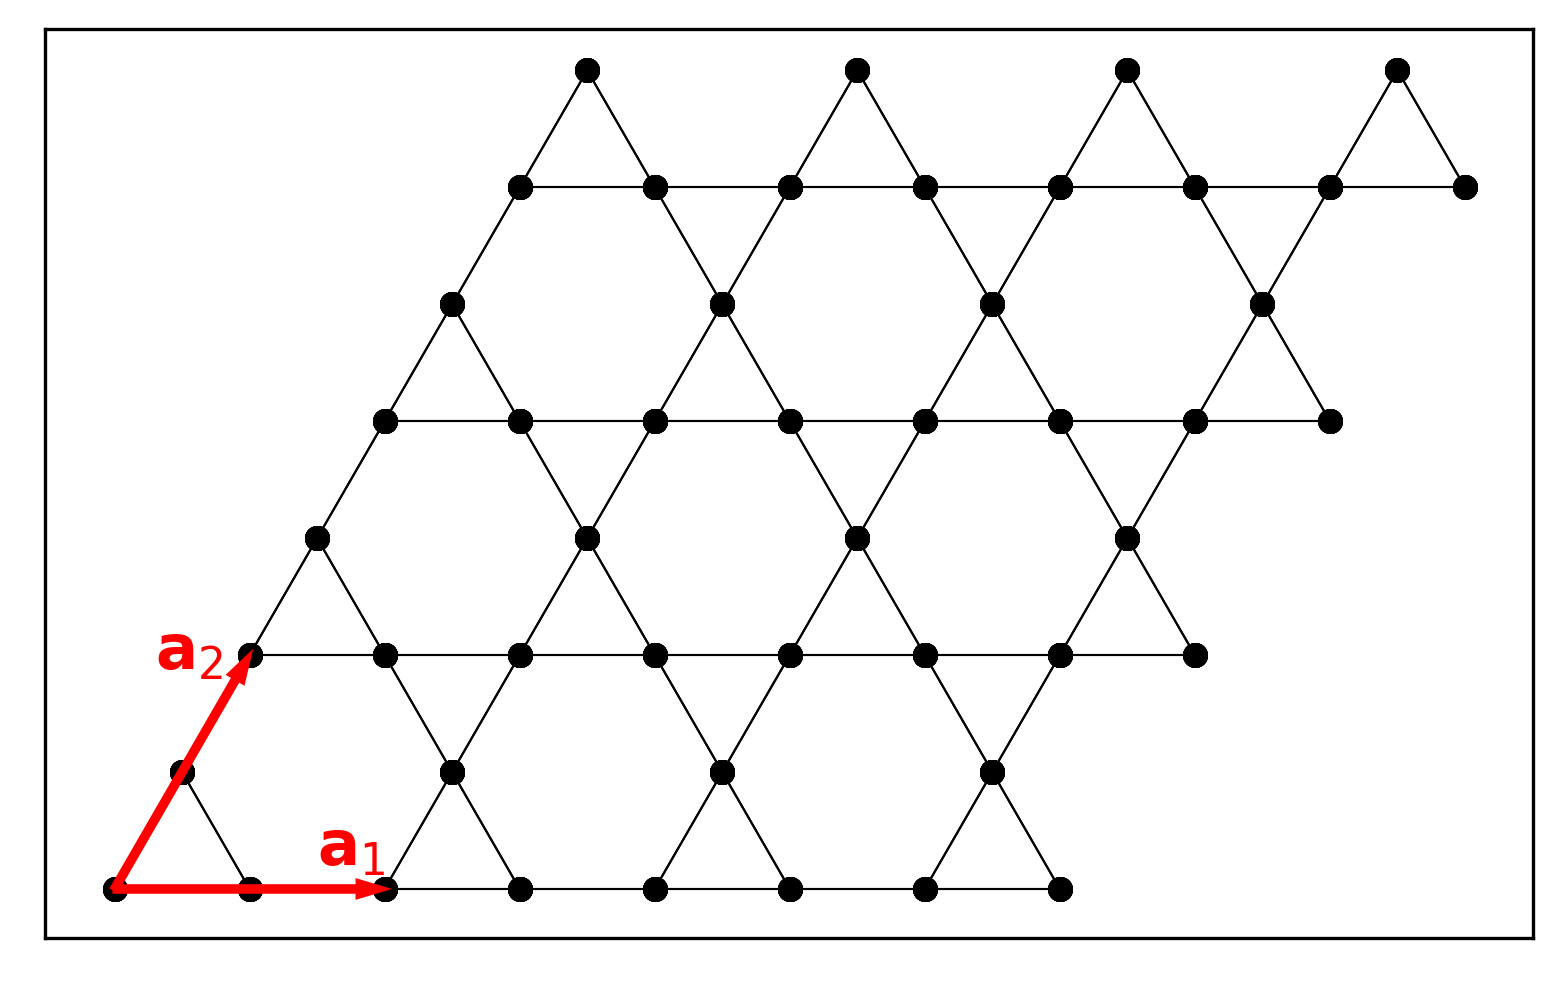
\includegraphics[width=0.42\textwidth]{Figures/Lattice_Structure}\label{Fig:Lattice_Structure}}\hfill
    \sidesubfloat[]{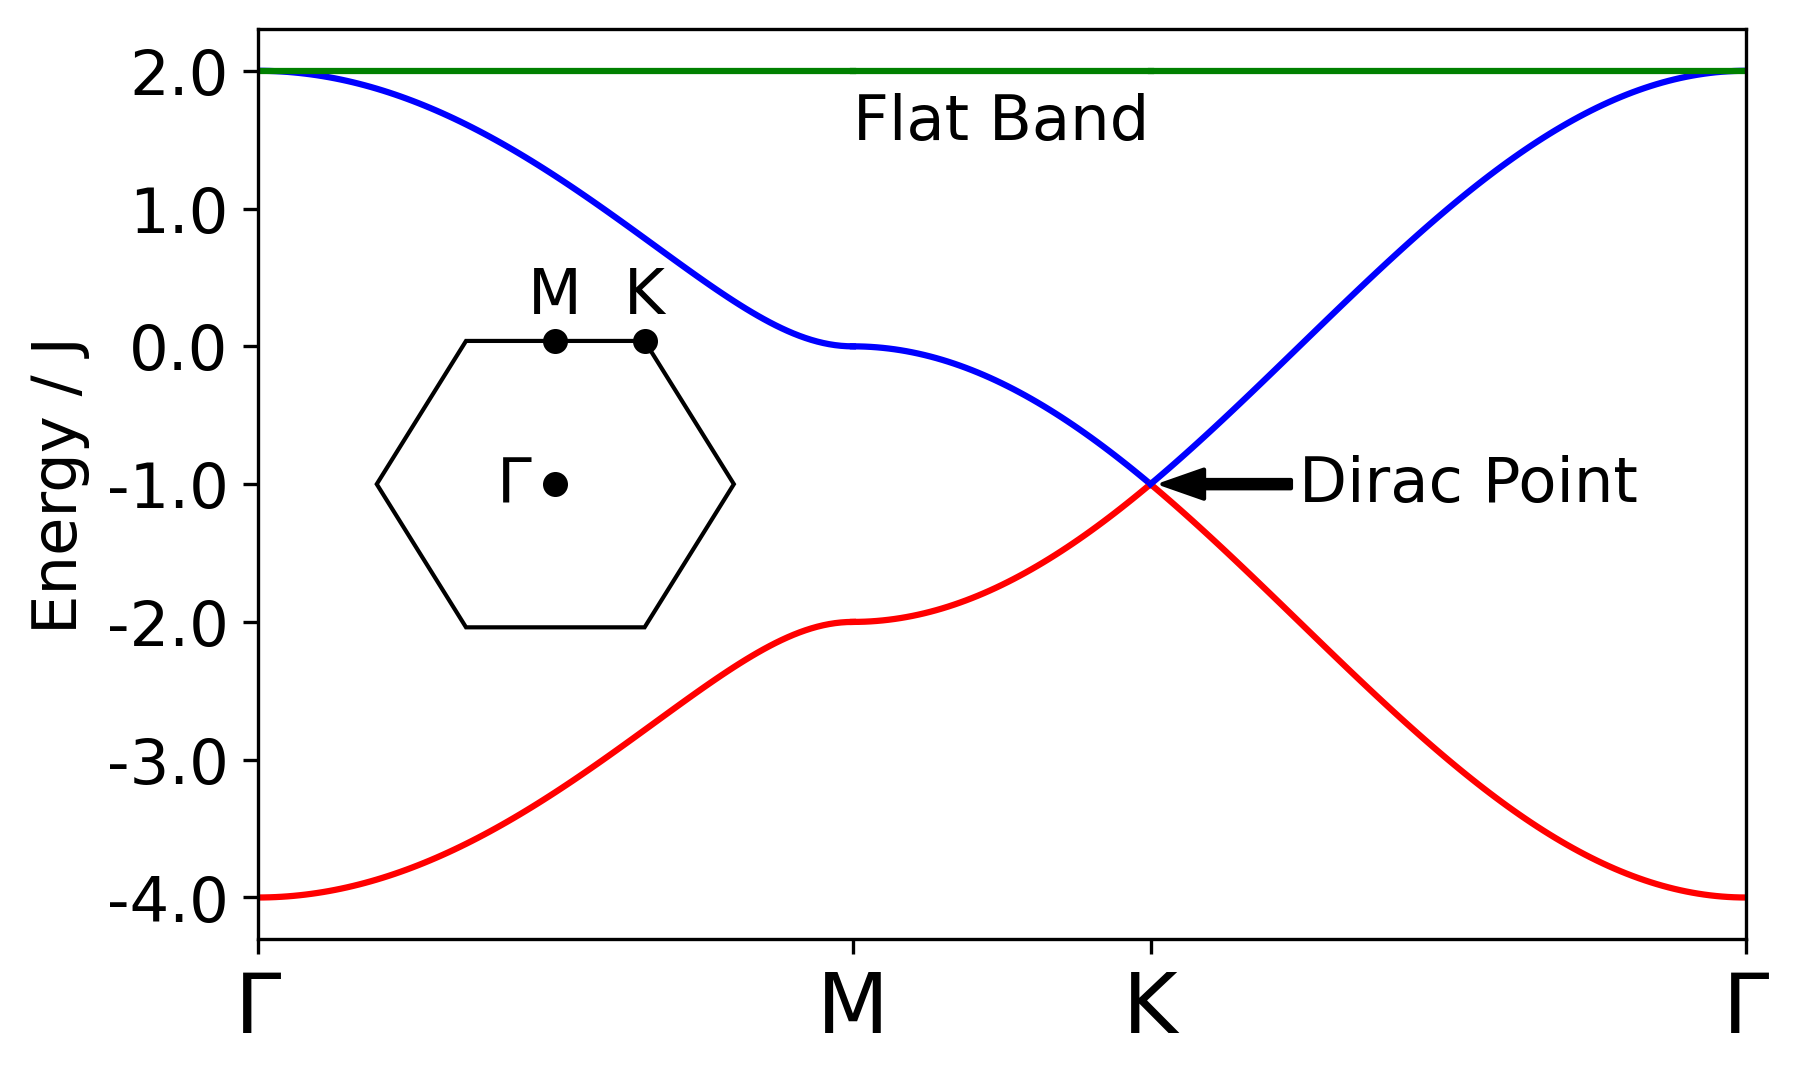
\includegraphics[width=0.48\textwidth]{Figures/Bandstructure}\label{Fig:Bandstructure}}
    \caption{(a) Kagome lattice section, with lattice vectors in red. (b) Single-particle bandstructure, with the first Brillouin zone inset. The highest-energy band (green) is flat.}
    \label{Fig:Lattice_and_Bandstructure}
\end{figure}

\vspace{0.75cm}

The single-particle bandstructure of the Kagome lattice (Fig. \ref{Fig:Bandstructure}) is obtained through a Fourier transform:
\begin{equation}\label{Eq:OperatorFT}
    b_{\textbf{k}\alpha}=\frac{1}{\sqrt{N_c}}\sum_{i}e^{-i\textbf{k}\cdot\textbf{r}_{i\alpha}}b_{i\alpha}
\end{equation}
where the sum runs over unit cells $i$ (not individual sites as in Eq. \ref{Eq:BHM}), the number of unit cells is $N_c$, and $\alpha$ indexes the three sites in the unit cell. The Hamiltonian becomes:
\begin{subequations}\label{Eq:MomentumBH}
\begin{equation}
H_J=\sum_{\textbf{k},\alpha,\beta} b_{\textbf{k}\alpha}^{\dag} \mathcal{H}_{\alpha \beta}(\textbf{k}) b_{\textbf{k}\beta}
\end{equation}
\begin{equation}
\mathcal{H}(\textbf{k}) = -2J
    \begin{pmatrix}
    0 & \cos k_3 & \cos k_2 \\
    \cos k_3 & 0 & \cos k_1 \\
    \cos k_2 & \cos k_2 & 0 
    \end{pmatrix}
\end{equation}
\end{subequations}
where $\textbf{k}$ is in the first Brillouin zone, $k_i=\textbf{k}\cdot\textbf{a}_i/2$ for $i=1,2$, and $k_3=k_2-k_1$. Diagonalizing $\mathcal{H}(\textbf{k})$ gives the three energy bands:
\begin{subequations}\label{Eq:BandEnergies}
    \begin{equation}\label{Eq:MobileBandEnergies}
        E_\textbf{k}^{(1,2)}=J(-1\pm\sqrt{4(\cos^2 k_1 + \cos^2 k_2 + \cos^2 k_3) - 3}
    \end{equation}
    \begin{equation}\label{Eq:FBEnergy}
        E_\textbf{k}^{(3)}=2J
    \end{equation}
\end{subequations}
The flat band eigenvector is:
\begin{equation}\label{Eq:FBEigenvector}
    \textbf{m}_{\textbf{k}}^{(3)}=\frac{1}{\sqrt{\sin^2 k_1+\sin^2 k_2 + \sin^2 k_3}}
    \begin{pmatrix}
        \sin k_3 \\
        -\sin k_2 \\
        \sin k_1
    \end{pmatrix}
\end{equation}
The dispersive band eigenvectors are not required in this project. The components of $\textbf{m}_{\textbf{k}}^{(3)}$, denoted $m_{\textbf{k}\alpha}^{(3)}$, define the single-particle flat band Bloch states:
\begin{equation}\label{Eq:FBBlochState}
    |\textbf{k}\rangle=\sum_{\alpha} m_{\textbf{k}\alpha}^{(3)} b_{\textbf{k}\alpha}^{\dag}|0\rangle
\end{equation}

The group velocity of particles is:
\begin{equation}\label{Eq:GroupVelocity}
    \textbf{v}_g=\frac{1}{\hbar}\nabla_{\textbf{k}}E_{\textbf{k}}
\end{equation}
Particles in the flat band are therefore stationary, with $\textbf{v}_g=0$. In the real-space picture, the extensive degeneracy of the flat band states enables the construction of spatially localised eigenstates. The most localised possible state is hexagonal (see Fig. \ref{Fig:Hexagon_Eigenstate}); the localisation can be intuitively understood as arising from destructive interference preventing hopping outside the hexagon. Non-overlapping hexagons form many-particle flat band eigenstates; however, the hexagons are not orthonormal, and cannot be used as a basis for the flat band \cite{Huber}.

For Hubbard systems with a single fermionic species, the behaviour is effectively non-interacting since the Pauli principle forbids multiple occupancy of any site. Past numerical simulations of such systems have confirmed that particles in dispersive bands are mobile, whereas particles in flat bands remain stationary indefinitely \cite{Chien14-1,Apaja,Hyrkas}.

\newpage

\begin{figure}[ht!]
    \centering
    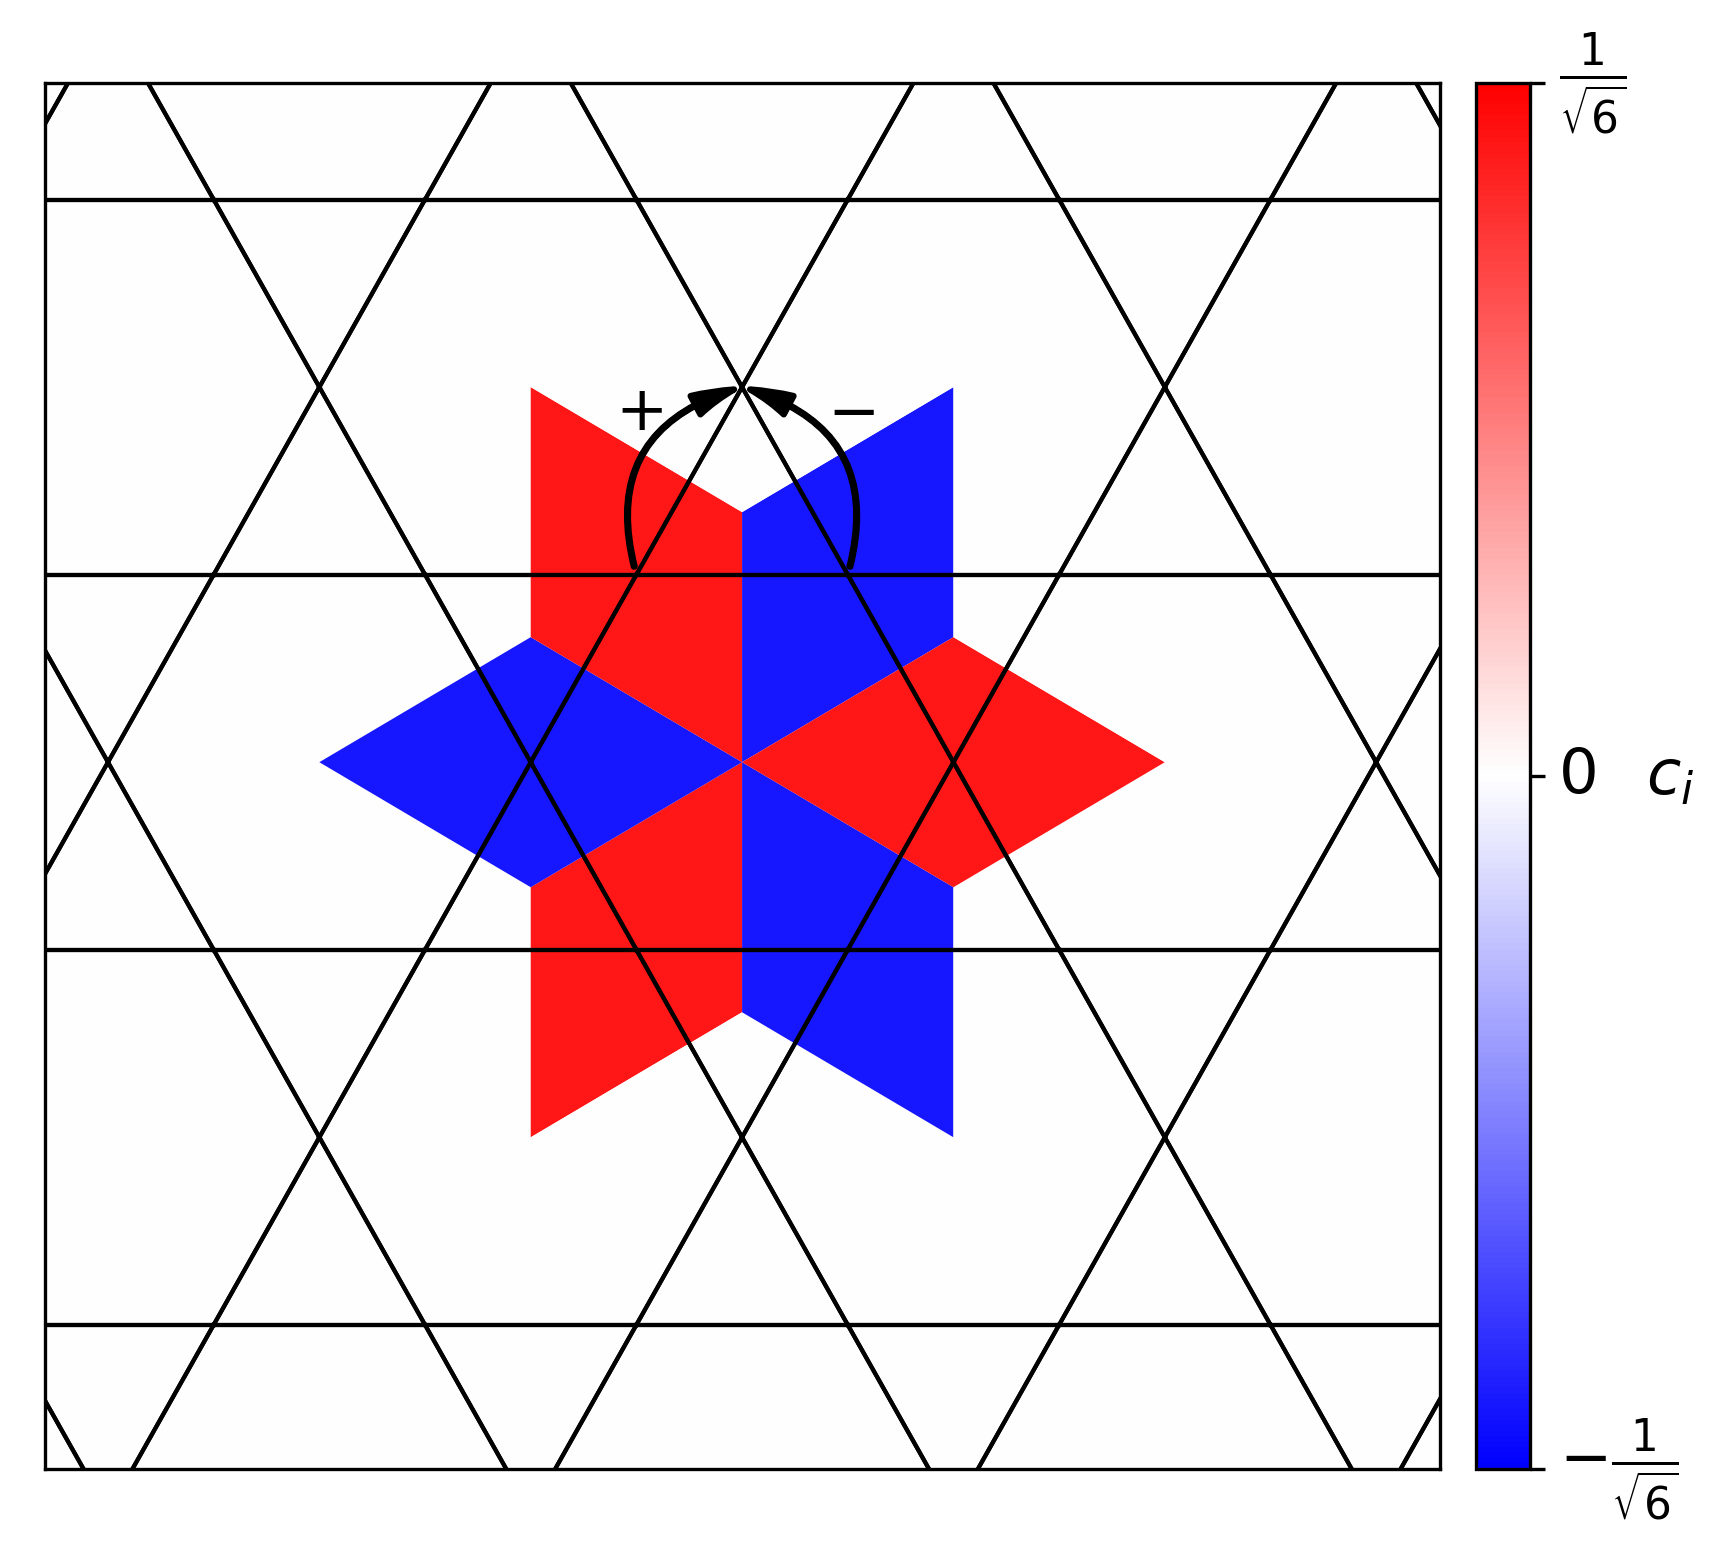
\includegraphics[width=10cm]{Figures/Hexagon_Eigenstate}
    \caption{Hexagonal flat band eigenstate. The amplitude of $|\Psi\rangle$ at each site, $c_i=\langle0|b_i|\Psi\rangle$, is shown.  Destructive interference between sites with opposite signs prevents hopping outside the hexagon, as illustrated. In this plot and others throughout the report, to eliminate blank space, the entire area closest to a given lattice site is coloured according to the value of the quantity being plotted (here, $c_i$) at that site.}
    \label{Fig:Hexagon_Eigenstate}
\end{figure}

\section{Interactions in Flat Bands}\label{Sec:WeakInteractionTheory}

For weak interactions, $U\ll J$, $H_U$ can be treated as a perturbation to $H_J$. Direct products of single-particle eigenstates are therefore good two-particle eigenstates, but with their eigenvalues shifted (in general) by the interaction energy. This partially lifts the degeneracy in the flat band, enabling particle mobility. However, for two single-particle flat band states with no real-space overlap, there is no interaction energy shift to the eigenvalues; the particles therefore remain stationary. Accordingly, particles are only expected to propagate in bound pairs.

In \cite{Torma}, expressions for the energy eigenvalues of bound particle pairs are derived in terms of the Bloch eigenvectors (Eq. \ref{Eq:FBEigenvector}), for systems with an isolated flat band (not strictly accurate for the kagome lattice, whose second band touches the flat band, see Fig. \ref{Fig:Bandstructure}). The energy shifts relative to the flat band are determined by the total momentum of the particles, $\textbf{q}=\textbf{k}_1+\textbf{k}_2$, and are proportional to $U$:
\begin{equation}
    \Delta E_{\textbf{q}} \propto U
\end{equation}
See Appendix \ref{App:Pair_Energy} for further mathematical details; the errors due to the isolated flat band approximation turn out to be minor. Although this theoretical framework exists, however, the interaction-shifted eigenspectrum, and the resulting dynamical behaviour, are yet to be determined for the kagome lattice.

The dynamical effects of interactions lifting the degeneracy in (non-kagome) flat band systems are investigated numerically in \cite{Apaja,Hyrkas}. Instead of remaining localized in flat band states like (effectively non-interacting) spinless fermions, bosons propagate from their initial state. These papers only cover the limiting case of $U\rightarrow \infty$. The qualitative interpretation that interactions break the flat band degeneracy, enabling transport, is the same as the weak-interaction case described above; however, neither the dependence of the behaviour on (finite) interaction strength, nor the kagome lattice specifically, are considered.

Cold atom experiments investigating Lieb \cite{Ozawa} and kagome \cite{Leung} systems have similarly found that interacting bosons in (formerly) flat bands acquire non-zero group velocities. This is explained as the interaction energy renormalizing the lattice potential energy within the Gross-Pitaevskii equation. In contrast to these many-particle, mean-field methods, this project adopts a few-particle, microscopic approach. Although the effect of interactions may be qualitatively similar in enabling transport, the details of the behaviour for the systems considered here are unknown.

\section{Strong-Interaction Regime}\label{Sec:DoublonTheory}

In the strong-interaction limit, $U \gg J$, the interaction energy far exceeds the maximum possible kinetic energy. With no dissipation mechanisms (as in cold atom experiments), particles on the same site cannot separate while conserving energy, and are therefore `repulsively bound' together as a `doublon'. Similarly, particles on separate sites cannot subsequently occupy the same site. The eigenspectrum of the system therefore splits into a high-energy doublon band, and a low-energy `scattering' band, with eigenstates composed of doubly- and singly- occupied sites respectively \cite{Valiente08,Deuchert}. Cold atom experiments, firstly \cite{Winkler}, have verified this theoretical prediction. 

The doublon band can be modelled by an effective single-particle Hamiltonian with an energy offset $E_0$ and hopping coefficient $J_{\text{eff}}$. Using second-order perturbation theory, these are given by \cite{Salerno}:
\begin{subequations}\label{Eq:DoublonHamiltonian}
    \begin{equation}
        H_{\text{eff}}=E_0 - J_\text{eff}\sum_{\langle ij \rangle} d_i^{\dag}d_j + \text{H.c.}
    \end{equation}
    \begin{equation}
        E_0 = \langle d_i |H|d_i\rangle + \sum_{s}\frac{|\langle s |H|d_i \rangle|^2}{E_{d}-E_{s}}=U + \frac{8J^2}{U}
    \end{equation}
    \begin{equation}
        J_{\text{eff}}=-\sum_{s}\frac{\langle d_j|H|s \rangle \langle s |H| d_i \rangle}{E_d - E_{s}}=-\frac{2J^2}{U}
    \end{equation}
\end{subequations}
Here, $d_i^{\dag}=\frac{1}{\sqrt{2}}(b_i^{\dag})^2$ creates a doublon on site $i$, $|d_i \rangle=d_i^{\dag}|0\rangle$, $|s \rangle$ is a virtual intermediate (scattering) state, and $H$ is the BH Hamiltonian (Eq. \ref{Eq:BHM}). The hopping amplitude has the opposite sign to Eq. \ref{Eq:BHM}. 

\section{Summary and Project Aims}\label{Sec:ProjectAims}

This section has presented the existing theory and research relating to dynamics in flat band systems, and the kagome lattice specifically. Without interactions, particles in flat band states are immobile; interactions lift the degeneracy of the flat band, enabling transport. Previous numerical and experimental research is all consistent with this general behaviour. Additionally, for strong interactions, a separation of doublon and scattering states is expected.

However, there is a lack of research into the specific subject of this project: the non-equilibrium dynamics of small numbers of bosons in a kagome lattice. Previous research has concerned either fermions \cite{Chien14-1}, different lattices \cite{Torma,Apaja,Hyrkas,Ozawa}, or mean-field cases \cite{Ozawa,Leung}; the details of the physics in the systems considered here are unknown. Moreover, the full range of interaction strengths has not been investigated.

In this report, different behaviour regimes are systematically investigated, developing a broad understanding of one- and two-boson kagome systems. Single-particle simulations are discussed in Section \ref{Sec:SingleParticleResults}, and quantitatively tested against the theoretical predictions from the single-particle bandstructure. Two-particle results are presented in Section \ref{Sec:TwoParticleResults}. The relationship between interaction strength and particle mobility is investigated and explained for states which, without interactions, would be stationary, localised flat band states. For strong interactions, the eigenspectrum of the system is compared to the theoretical predictions of Section \ref{Sec:DoublonTheory}, and the resulting dynamical behaviour examined.